\documentclass[output=paper]{langsci/langscibook} 
\ChapterDOI{10.5281/zenodo.1441335}
\author{Juan María Garrido Almiñana\affiliation{National Distance Education University}}
\title{Using large corpora and computational tools to describe prosody: An exciting challenge for the future with some (important) pending problems to solve}
\shorttitlerunninghead{Using large corpora and computational tools to describe prosody}

\abstract{This chapter presents and discusses the use of corpus-based methods for prosody analysis. Corpus-based methods make use of large corpora and computational tools to extract conclusions from the analysis of copious amounts of data and are being used already in many scientific disciplines. However, they are not yet frequently used in phonetic and phonological studies. Existing computational tools for the automatic processing of prosodic corpora are reviewed, and some examples of studies in which this methodology has been applied to the description of prosody are presented.}

\maketitle

% % Keywords
% % Computational tools; large corpora; prosody

\begin{document}\label{chap:gar2}\label{ch:1}

\section{Introduction}
The ``classical'' experimental approach to the analysis of prosody (questions and hypotheses, corpus design and collection, data measurement, statistical analysis, and conclusions) has until recently been carried out using mostly manual techniques. However, doing experimental research using manual procedures is a time-consuming process, mainly because of the corpus collection and measurement processes. For this reason, usually small corpora, recorded by a few number of speakers, are used, which is a problem if the results are supposed to be considered representative of a given language, for example.

Recent advances in speech processing techniques and computational power are changing the way in which experimental research in phonetics and phonology is done. These changes result in two main consequences: more storage capabilities, which allow for collecting and storing larger amounts of analysis material, and more powerful speech processing tools, which allow for the automation of some procedures. Many scientific disciplines, some of them related to speech and language, are exploiting the new challenges of processing large amounts of data in an automatic way (for example, Language and Speech Technologies, Text-to-Speech, Speech Recognition, Sentiment Analysis, Opinion Mining, Speech Analytics, and Corpus Linguistics). 

The ``big data'' approach to analysing raw data, which consists of using huge amounts of material to be analysed by applying fully (or almost fully) automatic processes and using powerful computational tools, is currently present in many disciplines, like marketing, advertising, and medical research. Its main advantages are evident: using large datasets leads to better predictions obtained in a faster and cheaper way than traditional methods. But they also have clear disadvantages: ``noise'' (wrong data) is present in the data, and, if it is too high, may lead to incorrect predictions. If the ``noise'' is low enough, however, the sheer amount of processed material can prevent it from influencing the data.

The goal of this work is to discuss to what extent it is now possible (or it will be in the near future) to apply ``big data'' methods to the analysis of prosody, by designing experiments with a large quantity of speech data representing a large number of speakers, processed in a fully automatic way with no manual intervention, and to obtain reliable and relevant results for prosodic research. It is evident that in the last decades some steps in this direction have been taken in prosody research, at least to analyse larger (and more representative) corpora using more complex (and more automatic) tools: new methods and tools are being introduced for corpus collection, corpus annotation, acoustic measurement and statistical analysis. 

In the next sections a review of the advances of these fields is given, with a special emphasis on some of the tools and methods developed and applied in our own research, which share as common feature the fact that they have been developed using a knowledge-based, linguistic approach for the automatic processing of speech. A brief description of how some of these tools work, and a discussion about their usefulness to automatically process large amounts of speech data, is also provided.

\section{Corpus collection}

Until quite recently, experimental research on prosody has involved the use of ``laboratory'' corpora, made up of \textit{ad hoc} material, specially designed and recorded for the experiment, uttered by a small number of speakers, and containing a reduced number of cases of the phenomena being studied. From an experimental point of view, the advantages of this kind of material are clear, mainly the high level of control of the variables affecting the analysed phenomena. However, it also has some drawbacks, such as the need for careful corpus design, which is usually a time-consuming task, and can sometimes lead to collecting unnatural material. Recording is also a slow and sometimes expensive procedure, in which volunteer or paid speakers must be recruited.

The use of ``real'' corpora, not specially designed for a specific experiment, can avoid these problems if they are large enough. Ideally, the phenomena to be studied (different sentence types, stress or rhythmic patterns and syntactic or information structures, for example) would be present in a representative number, and the experimenter should simply select the desired number of examples from the corpus to obtain a ``controlled'' experiment from more realistic material (see \citeauthor{Peskova.2018}, this volume). The whole corpus could even be processed and conveniently annotated with the information about the variables to be analysed without paying attention to the balance between the items representing each considered variable.

This approach is possible if the corpora are very large and contain hundreds of items that represent the variables to be analysed. This means many hours of collected speech (probably hundreds) must be annotated with the necessary information. How to obtain this kind of large and natural material arises, then, as an important methodological problem. Three possible ways to obtain larger corpora are: joint collections, corpus sharing, and the use of the Internet as a global corpus.

\subsection{Joint collection}\largerpage[-1]
Joint collection of corpora, by several research groups or individuals, is a possible way to obtain larger speech corpora for prosodic analysis. This can be done either through funded projects, in which several groups coordinate their efforts for the design, collection, and annotation of large corpora, or cooperative initiatives, in which volunteer contributions from many people enable the creation of databases in a collective (and cheaper) way.

One existing example of the first approach is the Glissando corpus \citep{Garrido2013Glissando}. Glissando is an annotated speech corpus specially designed for the analysis of Spanish and Catalan prosody from different perspectives (Phonetics, Phonology, Discourse Analysis, Speech Technology, and comparative studies). It includes two parallel corpora, \textit{Glissando\_sp} (Spanish) and \textit{Glissando\_ca} (Catalan), designed following the same criteria and structure: two subsets of recordings, representing two different speaking styles (news reading and dialogues), which were recorded in high-quality professional conditions by 28 different speakers per language, both professional and non-professional, which represents more than 20 hours of speech available per language. Both corpora were also orthographically and phonetically transcribed and annotated with different levels of prosodic information. These features make Glissando a useful tool for experimental, corpus-based, and technological applications. 

The Glissando corpus is the result of a publicly funded (Spanish Government) coordinated project of three different research groups: the Computational Linguistics Group (\textit{Grup de Lingüística Computacional}, GLiCom) from the Pompeu Fabra University and the Prosodic Studies Group (\textit{Grup d'Estudis de Prosòdia}, GrEP) from the Autonomous University in Barcelona, and the Group of Advanced Computational Environments – Multimodal Interaction Systems (\textit{Grupo de Entornos Computacionales Avanzados} - \textit{Sistemas de Interacción Multimodal}, ECA-SIMM), from Valladolid University. These three groups, with a common interest in prosody but coming from different research perspectives, worked together both in the design and the recording phases, taking advantage of their multidisciplinary backgrounds (both technical and linguistic). This coordinated work afforded the collection of a much larger corpus and with relevant annotation for different purposes.

The design procedure of Glissando is also an example of how to build a partially controlled corpus, in which phenomena that are potentially interesting for prosodic analyses have been included or induced in the corpus design from ``natural'' material, trying to keep a balance between naturalness and relevance. In the case of the news subcorpus, texts were not artificially built, but selected using automatic techniques from a larger set of real news texts, kindly provided by the \textit{Cadena SER} radio station, to obtain the best possible coverage in terms of (theoretical) intonation groups, stress patterns, and allophonic representation. Only in some specific cases were the original texts manually modified to ensure the presence of non-frequent cases (proparoxytone words, for example) in the corpus \citep{Escudero2009,Escudero2010}. In the case of the task-oriented dialogues subcorpus, several dialogue situations were designed to facilitate certain prosodically relevant interactions, for example, by asking a subject to obtain information which his/her dialogue partner could not provide, forcing an apology for this fact, and to change their dialogical strategies during the conversation. Finally, in the case of informal dialogues, dialogue couples that shared a common past were chosen, and they were asked to speak about these common memories in order to facilitate informal, emotional, and relaxed interactions.

Some other good examples of joint efforts to collect large, multilingual corpora for prosodic studies are the AMPER Project, which also involves many groups among the Romance space to collect a set of parallel corpora for intonation studies \citep{Contini2002,Contini2003}, or the C-ORAL-ROM initiative, an EU-funded project in which four different groups from four different countries collected a corpus of non-laboratory speech in French, Italian, Portuguese, and Spanish \citep{Cresti2005}. In this latter case, although the corpus was not specially conceived for prosodic analyses, some work was devoted to the annotation of prosodic breaks in the four corpora and to the validation of the annotations \citep{Danieli2004,Danieli2005}.

\subsection{Corpus sharing}

The use of multiple corpora is also a way to obtain larger amounts of data for experiments. There are many suitable corpora for the analysis of prosody which are available for reusing, some of them free of charge (as in the case of Glissando, distributed under a Creative Commons License). Some others are available for a fee (as with the Boston Radio News Corpus, for example; \citealt{Ostendorf1995}). There are also different institutions and initiatives in charge of collecting, hosting, and offering corpora for different purposes, both in America (LDC, \href{https://github.com/fahmidur/reciprosody/blob/master/README.md}{Reciprosody}) and Europe (\href{http://www.elra.info/en/}{ELRA}, \href{http://www.sldr.fr/}{SLDR/ORTOLANG}).

Finally, in order to make corpus reusing easier, it is important that the conventions with which corpora are annotated are as standardized as possible. Initiatives to develop standards for the annotation of prosody are still needed. An example of such effort is the proposal of an annotation scheme for prosodic events developed in the framework of the MATE project \citep{Klein1998}. There is still much work to do in this area, however.

\subsection{Internet as a corpus}

The Internet can be a source for data collection for prosody research, as it is already for other disciplines. There is a huge amount of speech material available on the net (radio and television broadcasts, podcasts, YouTube), although its use is usually restricted, due to legal and privacy issues (copyright, for example), and its quality may vary from media to media. There are, however, some public repositories of media data with an acceptable level of recording quality, such as the \href{http://www.europarl.europa.eu/ep-live/en/plenary/search-by-date}{European Parliament session archives}, which have already been used for several research purposes, such as the development of speech-to-speech translation systems. Most of this material provides examples of formal speech, but informal material is more difficult to obtain (and process). YouTube can be a good source for this kind of material, if copyright problems are solved, but in this case the background noise can be a problem for automatic tools, especially in F0 estimation.

\section{Corpus transcription, segmentation, and annotation} 

Speech corpora need to include transcription and annotation to be useful for research purposes. For prosodic analysis, several types of information should ideally be available, both phonetic/phonological (phonetic or phonological transcription, prosodic phrasing) and linguistic (part-of-speech (POS), parsing, sentence type, speech acts, new/given information, focus, etc.), or paralinguistic (emotions, for example) events. The transcription and annotation of large corpora with all of this information is a task that cannot be done manually, so automatic tools are needed for the different tasks of transcription and annotation. The following subsections present a review of current tools for carrying out these tasks (orthographic and phonetic transcription and segmentation, prosodic unit segmentation, annotation of prosodic events, and annotation of linguistic information), with a special focus on two tools developed as part of our research, SegProso and MelAn.

\subsection{Automatic orthographic transcription and segmentation}

Orthographic transcription of oral material has traditionally been a problem for the collection of oral corpora. It is usually done by manual transcribers, who spend a large quantity of time on this task and may introduce transcription errors. Speech recognition technology (which allows for the automatic conversion of a speech signal into its corresponding orthographic transcription, by comparing the speech input to a set of acoustic models representing the phones of the input language) may be a faster alternative to face the task. However, the current performance of this technology is not accurate enough to obtain reliable transcriptions, especially with spontaneous, disfluent or noisy speech, as the acoustic models of these systems have been usually trained only with formal, clean speech, and their pronunciation dictionaries do not usually consider pronunciation variants that are atypical for standard speech (i.e. they show poor out-of-domain performance). Despite these problems, this kind of technology could provide a first automatic transcription that human reviewers could revise later, a task which would be faster than manually transcribing all of the material.

However, audio transcription tools using speech recognition technology (both public domain and commercial) do not seem to be available for this kind of task. Some existing tools do this job for other purposes, such as video caption tools (for example, the \href{https://support.google.com/youtube/answer/3038280?hl=en}{Youtube} captioning tool, from Google) or speech-to-speech translation tools (such as \href{https://support.google.com/translate/answer/6142468?hl=en}{Google Translate} or \href{http://www.skype.com/en/translator-preview/}{Skype Translator}). However, it is difficult to convert the output of these programs into a plain text transcription of input speech.

\subsection{Phonetic transcription and segmentation}

Manual phonetic transcription of corpora from directly listening to speech waves is an even more time-consuming task than orthographic transcription. In addition, it has to be done by human transcribers with a good background on phonetic transcription of the language, a much more specialised knowledge than the one needed to orthographically transcribe speech. Phonetic transcription of large corpora appears then to be an unaffordable task by manual means.

In this case, however, technology is already providing automatic alternatives for the phonetic transcription of speech, at least for some languages, if the orthographic transcription is provided. Phonetic aligners are tools that enable researchers to obtain a time-aligned phonetic transcription of a speech file, if an orthographic transcription of the speech wave is available. These tools are actually the result of merging two different speech technologies: automatic phonetic transcription of text, and automatic speech recognition. They usually work in two phases: first, the phonetic transcription is generated from the orthographic text, then the speech recognizer tries to align the obtained transcription with the speech wave, a task that is easier than simply trying to ``guess'' the phones of the speech chain using only a speech recogniser. 

Several public domain phonetic aligners are available on the net, such as \href{http://www.bas.uni-muenchen.de/Bas/BasMAUS.html}{MAUS} \citep{Schiel1999}, \href{https://clarin.phonetik.uni-muenchen.de/BASWebServices/index.html}{WebMAUS},  \href{http://latlcui.unige.ch/phonetique/easyalign.php}{EasyAlign} \citep{Goldman2011} or \href{http://www.sppas.org/}{SPPAS} \citep{Bigi2015}. \mbox{SPPAS} is a tool developed at the \textit{Laboratoire Parole et Langage} (Aix-en-Provence, France), which allows for phonetic transcription and alignment in several languages (Catalan, French, English, Spanish, Italian, Japanese, Mandarin, Chinese, and Cantonese). In addition to time-aligned phonetic transcription, it also allows for obtaining other automatic annotations, such as syllable segmentation, intonation group, or intonation annotation using MoMel \citep{Hirst1993}. Written in Python, it provides as output a Praat \citep{Boersma.praat} TextGrid file containing several tiers with the different levels of segmentation analysis. \figref{fig:gar:1} provides an example of this output for a sample Spanish sentence.

  
%%please move the includegraphics inside the {figure} environment
%%\includegraphics[width=\textwidth]{GAR-img15.png}
 

\begin{figure}
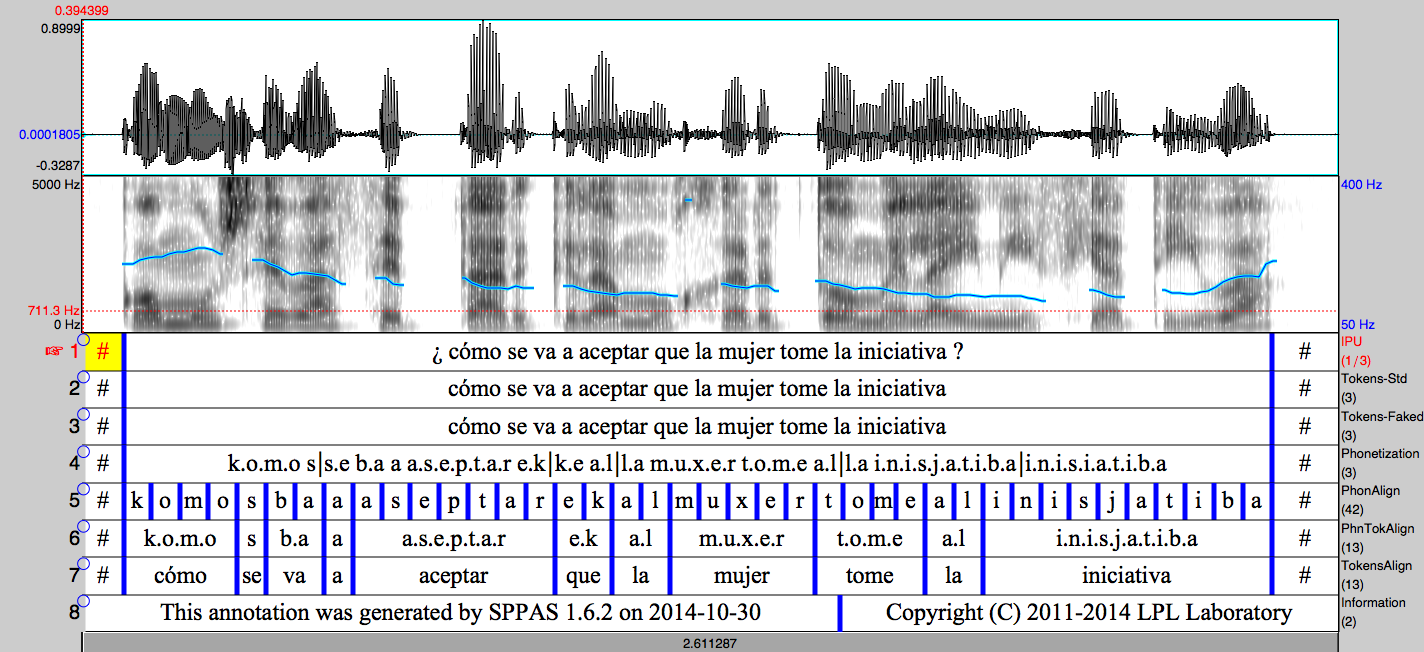
\includegraphics[width=\textwidth]{figures/GAR-img001.png}
\caption{TextGrid file containing the phonetic transcription (in SAMPA symbols) and prosodic annotation obtained with SPPAS for the utterance \textit{¿Cómo se va a aceptar que la mujer tome la iniciativa?} uttered by a female speaker of Spanish.}
\label{fig:gar:1}
\end{figure}

The Catalan and Spanish acoustic models necessary for the speech alignment phase have been trained using an annotated version of the Glissando corpus. For automatic phonetic transcription, SPPAS includes a phonetic dictionary for each available language, although it can be customised to use any dictionary or phonetic transcriber for this task.\largerpage

The main problem of these tools is that they provide the ``theoretical'' transcription of the input speech, not the actual pronunciation of the speaker, as they are based on the automatic transcription of the text, not on the acoustic analysis of the phones which make up the speech chain. The reliability of these tools is far from being perfect, but it seems good enough to process large amounts of data. In the case of SPPAS, for example, \citet{Bigi2012SPPAS} presents the results of an evaluation of the French aligner using three different corpora, AixOx, Grenelle, and CID, and the error rate of phonetisation errors moves between 8.8\% and 14.5\%. Apart from phonetisation errors, misplacements of phone boundaries can also appear. This gives poorer results than desired, which makes a later phase of manual review of the output necessary, a task which is much faster than a fully manual transcription from scratch.

\subsection{Automatic segmentation of prosodic units}

Prosodic phrasing annotation (marking prosodic unit boundaries, such as syllables or intonation units) has also been a traditional bottleneck in prosody studies. One reason for this is the lack of a common list of prosodic units across models and approaches in prosodic phonology: some units, such as syllables or intonation groups, are generally accepted, but there is less consensus about the definition or name of others (intermediate phrase, phonological word, stress group, or foot, for example). But it can also be due to the difficulty of the annotation task itself: it is known, for example, that human annotators show only reasonably high agreement levels in the task of intermediate phrase boundary detection (see \citealt{Syrdal2000}, among others), in addition to the fact that it is a very time-consuming task when done by humans, as in the case of the previously reviewed transcription tasks.

Previously mentioned tools (EasyAlign, SPPAS) allow, in addition to automatic phonetic transcription, the automatic annotation of some prosodic boundaries, such as syllables or intonation groups. However, some other public domain tools specifically oriented to this task are also available, such as APA (for the automatic identification of syllable and tone unit boundaries; see \citealt{Cutugno2002} or \citealt{Petrillo2004}), Analor (which provides tone unit segmentation; \citealt{Avanzi2008}) or SegProso (for the annotation of syllables, stress groups, intonation groups, and breath groups; \citealt{Garrido2013SegProso}). SegProso is actually a set of Praat scripts which add to an input TextGrid file which contains the orthographic and phonetic transcription of the utterance and four new tiers with the prosodic unit segmentation. Originally designed for the annotation of speech in Spanish and Catalan, SegProso was later extended to Brazilian Portuguese and Mandarin Chinese, and more recently, to French. \figref{fig:gar:2} presents an example of this tool’s output, in Praat TextGrid format. SegProso needs, as input, a wav file and its corresponding orthographic and phonetic transcription in a TextGrid file.

\begin{figure}
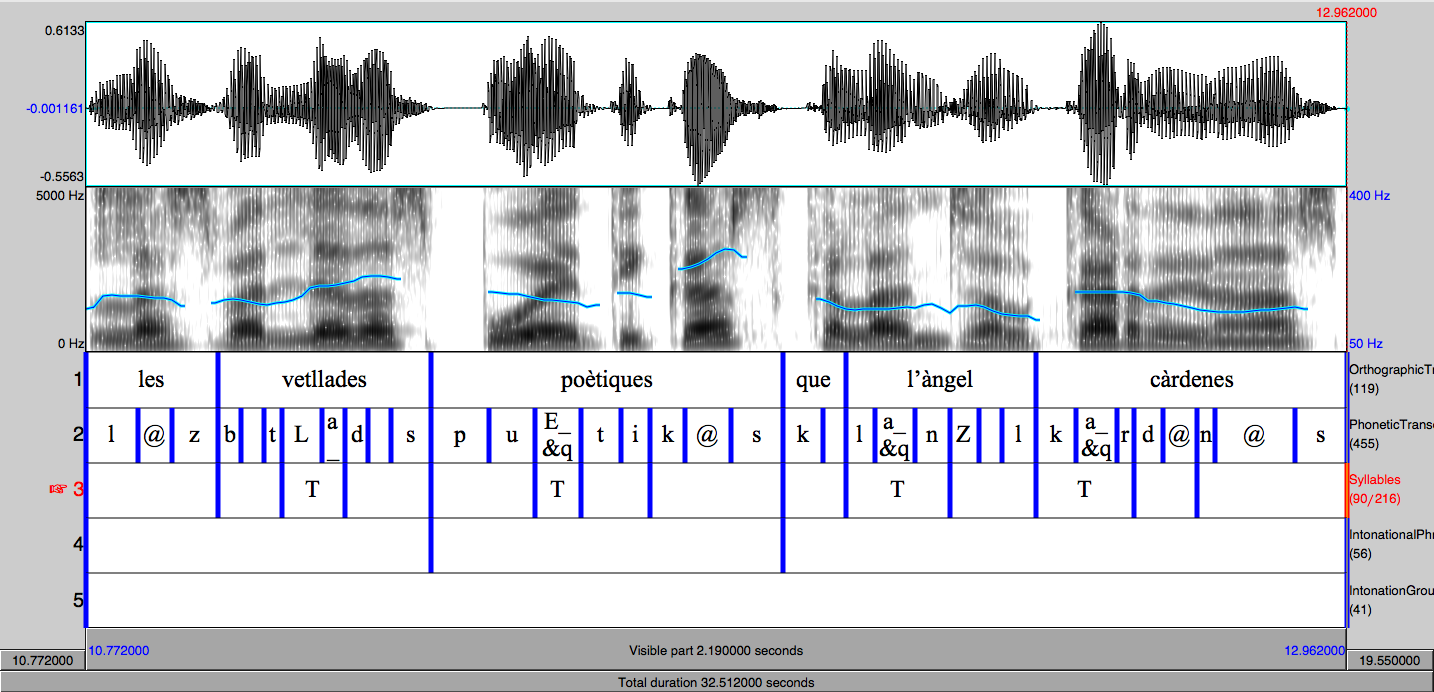
\includegraphics[width=\textwidth]{figures/GAR-img002.png}
\caption{TextGrid and waveform corresponding to the utterance ``les vetllades poètiques que l’Ángel Cárdenas", spoken by a female professional speaker.}
\label{fig:gar:2}
\end{figure}

Automatic tools for the identification of prosodic boundaries are built either using data-driven (automatic creation of models from the analysis of large sets of annotated data) or knowledge-based techniques (using linguistic and phonetic rules manually developed by experts). Knowledge-based tools may approach this task from two different perspectives:

\begin{itemize}
\item In the first, acoustical approach, prosodic boundaries are detected from the acoustic analysis of the signal. For the detection of intonation unit boundaries, for example, APA and Analor try to identify acoustic cues such as pauses and boundary tones; APA tries to detect syllables by searching acoustic indices of syllabic nuclei; and finally, SegProso looks for relevant F0 movements for the identification of intermediate phrases and F0 resets, an acoustic cue that has also been claimed to be an indicator of the presence of prosodic boundaries (\citealt{Garrido1996,Garrido2001}, among others). 
 
\item In the second approach, the prosodic annotation is carried out by taking advantage of previously obtained annotations, mainly phonetic transcription. For syllable annotation, for example, SegProso uses the phonetic transcription provided as input, which must contain information about the location of the (theoretically) stressed syllables to determine syllable boundaries by means of a set of ``phonological'' rules which predict how phonetic symbols must be grouped; a similar approach is used for the annotation of stress groups (their boundaries are established using both the syllable limits previously derived from the phonetic transcription and the information about stressed vowels available in the phonetic transcription tier) and intonation groups (boundaries are derived from the pause information present in the phonetic transcription).
\end{itemize}

The approach based on the use of previously derived annotations seems to be, in general, more reliable than the first one, as it can be inferred from the results of the evaluation of SegProso with Spanish and Catalan data presented in \tabref{tab:gar:1} and \ref{tab:gar:2} \citep{Garrido2013SegProso}. The goal of the evaluation was to check to what extent the tool is able to correctly place prosodic unit boundaries in a small automatic annotation task. A set of 100 utterances for each language was selected as an evaluation corpus. The results of the evaluation showed an excellent performance of the syllable and breath group scripts for both languages (whose rules make annotations from previously obtained annotation tiers), a slightly lower performance rate in the case of stress group annotation (derived also from the phonetic transcription), and a lower performance of the intonation group script (whose rules detect potential boundaries from the acoustic analysis of the F0 curves). The lower performance of the stress group detector illustrates the risks of the first approach, as almost all the errors were due to errors in the annotation of the stressed vowels in the phonetic transcription tier, which had been also generated by automatic means. The lower performance of the intonation group detector shows that work still needs to be done to improve the acoustic detection of prosodic boundaries, although, in this case, the results are good enough to consider that they can be used as a starting point for a second phase of manual revision.

\begin{sidewaystable}\small
\begin{tabularx}{\textwidth}{X QQQQQQQQ}
\lsptoprule
Unit & N of boundaries (automatic version) & N of boundaries (revised version) & Correct boundaries & Moved boundaries & Deleted boundaries & Added boundaries & Pct. of correct boundaries (automatic version) & Pct. of actual boundaries correctly predicted \\
\midrule
Syllables & 1824 & 1824 & 1824 & 0 & 0 & 0 & 100 & 100 \\
\tablevspace
Stress groups & 568 & 568 & 496 & 72 & 0 & 0 & 87.32 & 87.32 \\
\tablevspace
Intonation groups & 308 & 297 & 254 & 21 & 33 & 22 & 82.46 & 85.52 \\
\tablevspace
Phonic groups & 122 & 122 & 122 & 0 & 0 & 0 & 100 & 100 \\
\lspbottomrule
\end{tabularx}
\caption{Results for the evaluation of the Spanish corpus \citep{Garrido2013SegProso}}
\label{tab:gar:1}
\end{sidewaystable}

\begin{sidewaystable}\small
\begin{tabularx}{\textwidth}{Q QQQQQQQQ}
\lsptoprule
Unit & N of boundaries (automatic version) & N of boundaries (revised version) & Correct boundaries & Moved boundaries & Deleted boudaries & Added boundaries & Pct. of correct boundaries (automatic version) & Pct. of actual boundaries correctly predicted \\
\midrule
Syllables & 1574 & 1574 & 1574 & 0 & 0 & 0 & 100 & 100 \\
\tablevspace
Stress groups & 628 & 628 & 543 & 85 & 0 & 0 & 86.46 & 86.46 \\
\tablevspace
Intonation groups & 354 & 323 & 274 & 31 & 49 & 18 & 77.40 & 84.82 \\
\tablevspace
Phonic groups & 168 & 168 & 168 & 0 & 0 & 0 & 100 & 100 \\
\lspbottomrule
\end{tabularx}
\caption{Results for the evaluation of the Catalan corpus \citep{Garrido2013SegProso}}
\label{tab:gar:2}
\end{sidewaystable}


\subsection{Prosodic annotation} 

The annotation of prosodic phenomena (intonation, stress, and tone) presents similar problems to prosodic units, such as the lack of a common inventory of annotation symbols, or the existence of several prosodic and metrical theories. In the case of intonation, ToBI \citep{Silverman1992} is largely used by people working in the framework of the autosegmental model for phonological prosodic analysis, but there are other conventions which have been used outside this framework, such as MoMel/INTSINT \citep{Hirst2000}, the IPO model (\citealt{Hart.1990}; \citealt{Garrido1996}), or Speech Melodic Analysis (\textit{Análisis Melódico del Habla}, \citealt{Cantero2009}).

Until very recently, the annotation of intonation events has been carried out manually, and consequently, has been very time consuming. Probably the first automatic tool for the annotation of intonation curves was MoMel, developed by Daniel Hirst and Robert Espesser at the \textit{Laboratoire Parole et Langage} of Aix-en-Provence, France (\citealt{Hirst1993}). 
In the case of ToBI, some automatic annotation tools have recently appeared, such as AuToBI \citep{Rosenberg2010} 
or Eti-ToBI (\citealt{ElviraGarcia2015}), or are still in development (\citeauthor{Escudero2014a} \citeyear*{Escudero2014a,Escudero2014b,Escudero2014c}; \citealt{Gonzalez2014}). 
Outside the ToBI framework, there are also some tools which implement other models of prosodic representation, such as the one developed by Mateo to implement the Speech Melodic Analysis annotation system \citep{MateoRuiz.2010protocolo,MateoRuiz.2010Scripts}, or MelAn \citep{Garrido2010}.

MelAn is an automatic tool for stylisation, annotation, and modelling of intonation contours, which is an automatic implementation of the intonation modelling framework presented in \citep{Garrido1996,Garrido2001}, inspired by the IPO model. According to this model, F0 contours are made up of a set of relevant inflection points that can be assigned to a high (Peak, P) or low (Valley, V) tonal level, as can be observed in \figref{fig:gar:3}. Two more symbols for extra high (P+) and extra low (V\textminus) levels are also used. It is then a phonetic annotation tool, in the sense that it does not try to capture the phonological tones behind the F0 curves, rather the pitch movements which are relevant from an acoustic-perceptual point of view, a much more feasible goal for an automatic tool at the current state of the art.\largerpage[-2]


\begin{figure}
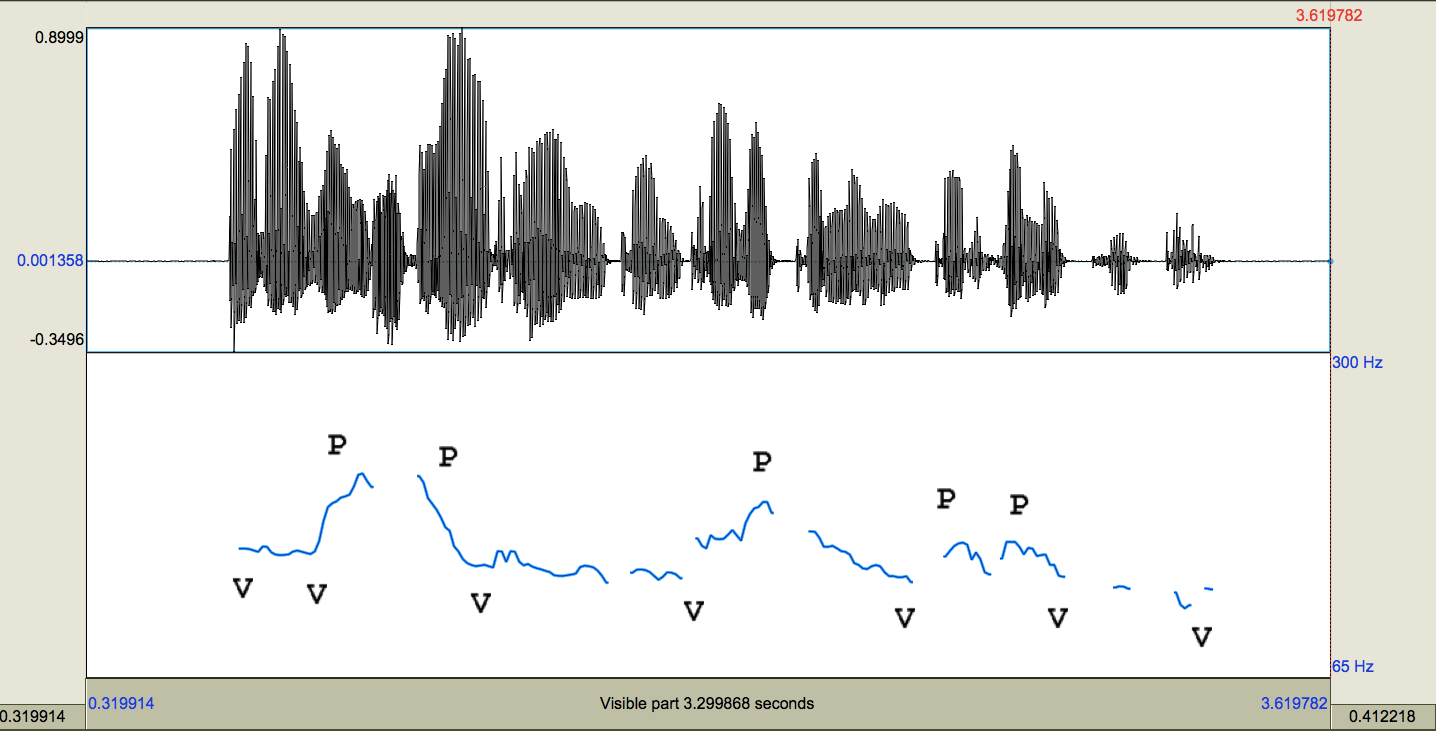
\includegraphics[width=\textwidth]{figures/GAR-img003.png}
\caption{Waveform and annotated F0 contour for the utterance \textit{Aragón se ha reencontrado como motor del equipo}, uttered by a female speaker of Peninsular Spanish. Relevant inflection points are marked with P and V labels, following the intonational annotation conventions described in \citet{Garrido1996,Garrido2001}.}
\label{fig:gar:3}
\end{figure}

MelAn performs the annotation procedure in two stages: stylisation, in which the original F0 trace is reduced to a set of relevant inflection points using the Praat stylisation functionality; and annotation, in which the obtained inflection points are annotated with a label indicating the relative height of the F0 value within the tonal range of a breath group. At the end of this process, both F0 values at the inflection points and intonation labels are stored in a TextGrid as the one presented in \figref{fig:gar:4}.

  
\begin{figure}
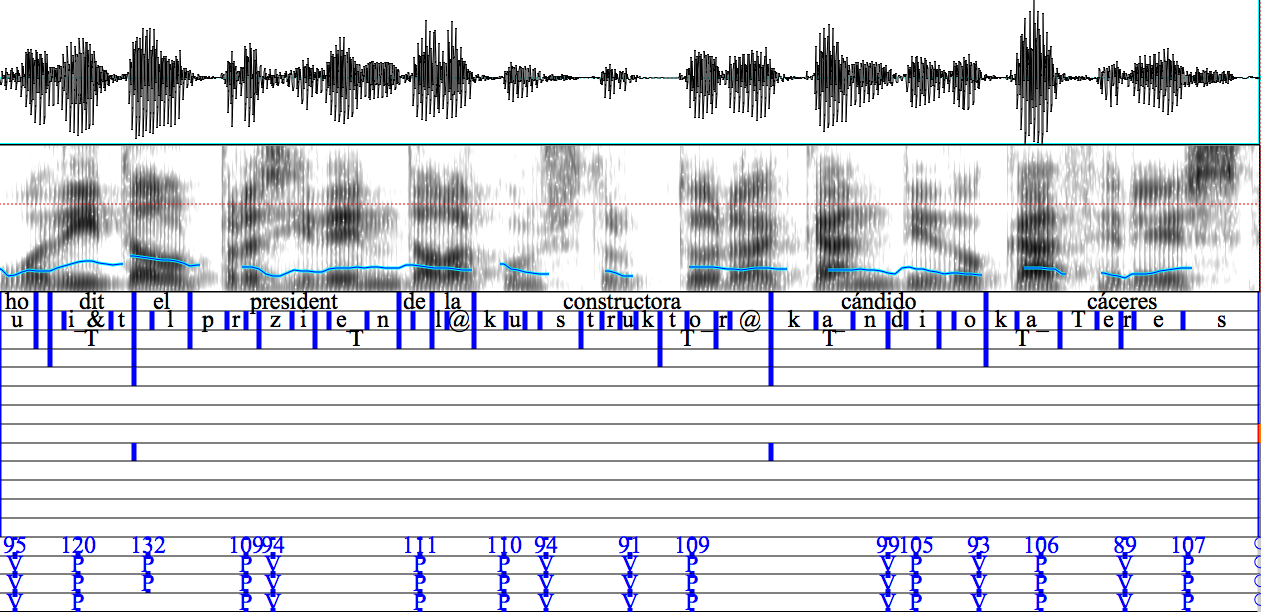
\includegraphics[width=\textwidth]{figures/GAR-img004.png}
\caption{Waveform, F0 contour, spectrogram and annotation of the utterance \textit{ho ha dit el president de la constructora, Cándido Cáceres}, uttered by a speaker of central Catalan. The last four tiers in the TextGrid present the output obtained with MelAn.}
\label{fig:gar:4}
\end{figure}
 

As stated before, the ideal goal of this kind of phonetic annotation tool is that the obtained labels are able to capture the relevant movements for the transmission of intonational information from the original F0 contour, rather than to capture phonological, linguistically relevant tonal events. In order to analyse to what extent MelAn meets this requirement, several perceptual evaluations were carried out to determine to what extent the annotated representation of F0 contours can be used to recover the original F0 trace, or at least to obtain a similar one, perceived close enough to the original one by native listeners of the analysed language. The procedure was the same in all cases: listeners had to listen to pairs of synthesized stimuli, both obtained from the same utterance, the first one generated with the original F0 contour and the second one generated with a simplified F0 contour derived from a symbolic MelAn representation, and rate the degree of similarity between them. This process of resynthesis was done using ModProso, another Praat-based tool developed for this purpose \citep{Garrido2013ModProso}. Figures~\ref{fig:gar:5} and \ref{fig:gar:6} present an example of one of these pairs for a Spanish utterance. 

 

As shown in \tabref{tab:gar:3}, the final global score was around 4 on a 1--5 scale, that is, a quite acceptable similarity between both contours, both for Spanish and Catalan. Similar results were obtained for other languages such as Mandarin Chinese (\citealt{Yao2010}), as shown in \tabref{tab:gar:4}, or Brazilian Portuguese (\citealt{ConceicaoSilva.2016}). These results seem to indicate that MelAn generates symbolic representations of F0 contours that are very similar in perceptual terms to the original ones in all of the analysed languages, some of them quite far away from a typological point of view. 

Additionally, it can also be useful to automatically annotate prosodic corpora with tonal events if the goal is to capture perceptually relevant movements. Of course, as the results of the evaluation also show, the symbolic annotation obtained may contain errors in some cases, which lead to a poorer rate in the perceptual evaluation task. These errors may come from different sources (errors in the estimation of the F0 curve, errors in the stylisation process, or errors in the assignment of the P/V label to a specific inflection point), but they do not seem to be frequent enough to provide an annotation that can be considered unacceptable. And again, if a more accurate annotation is needed, it can be manually corrected by a human expert.

 \begin{figure}[p]
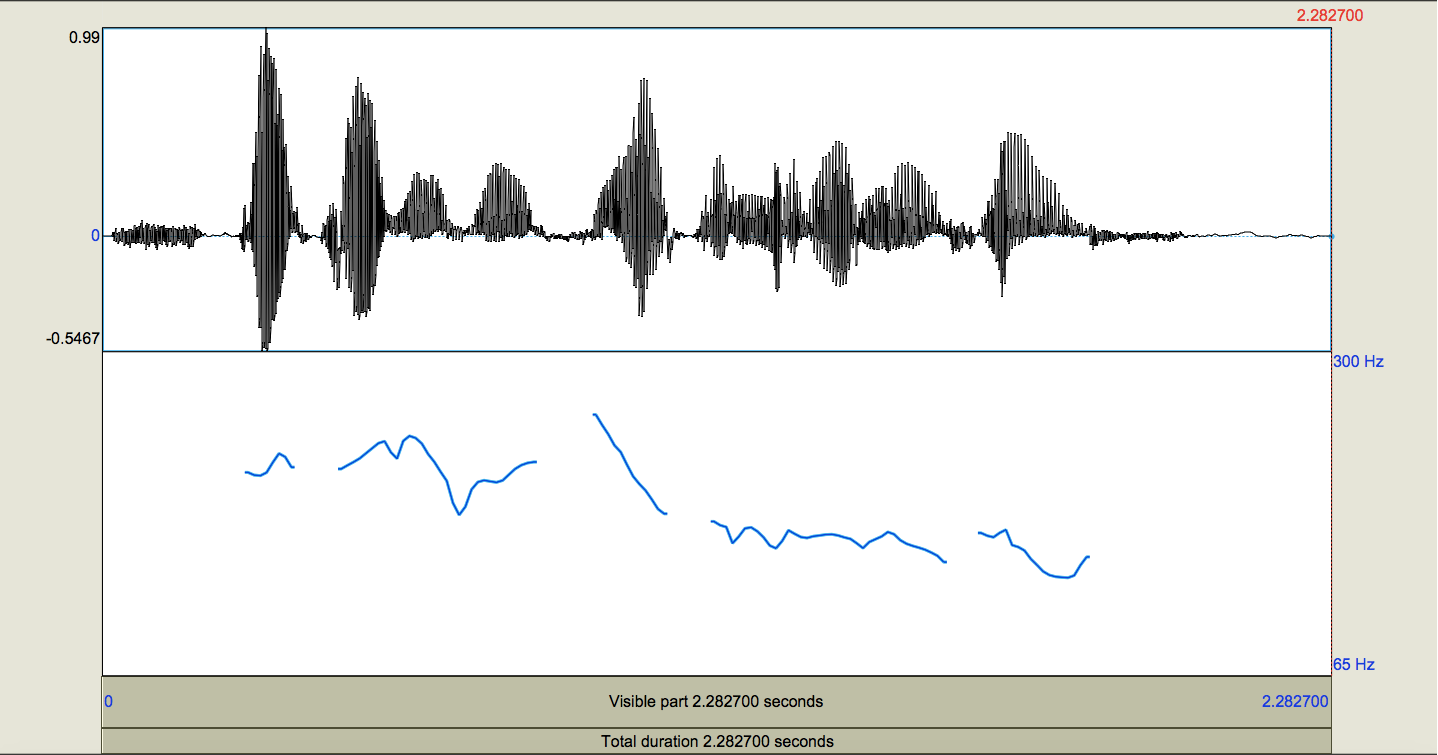
\includegraphics[width=\textwidth]{figures/GAR-img005.png}
\caption{Waveform and F0 contour of the synthesised version of the utterance \textit{Y cada vez la tendremos más}, uttered by a Spanish female speaker. The F0 contour used to generate this version is the original one.}
\label{fig:gar:5}
\end{figure}

 
\begin{figure}[p]
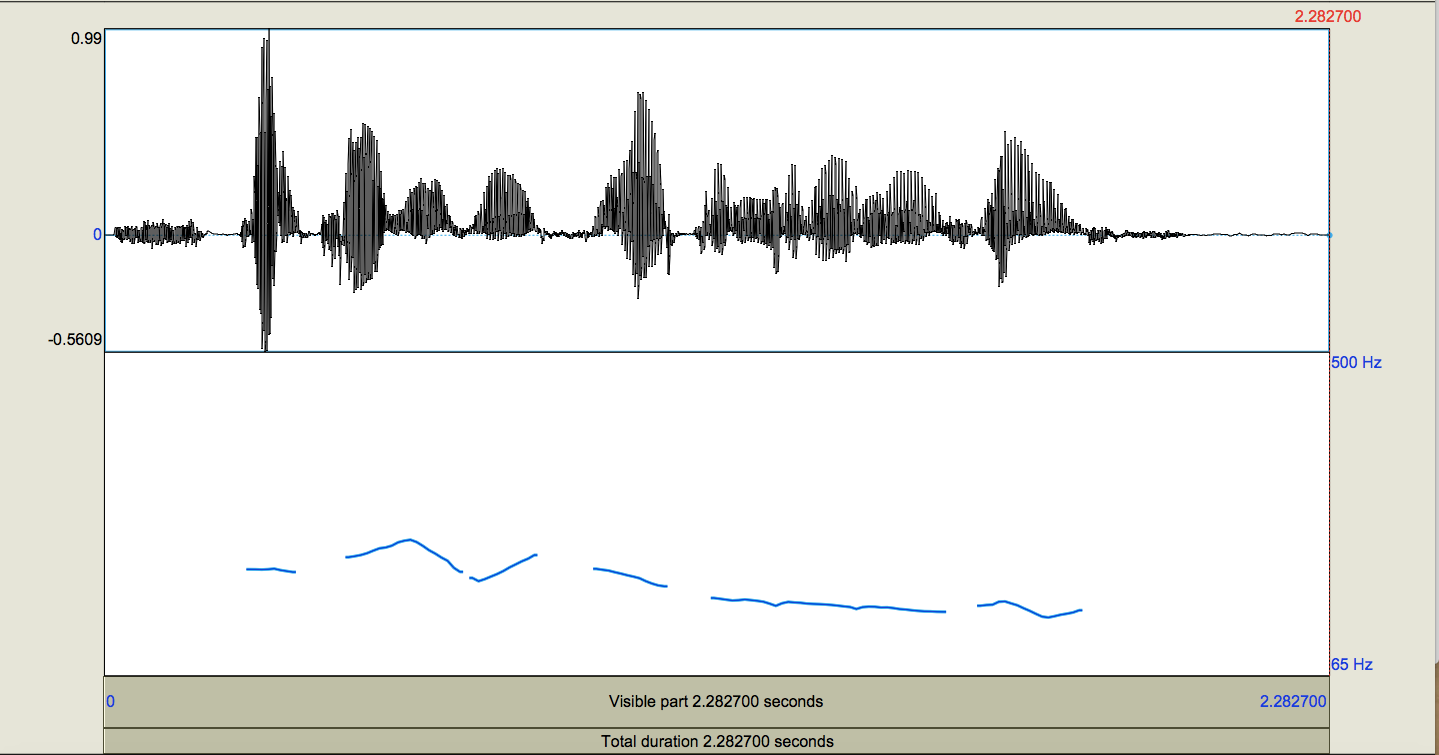
\includegraphics[width=\textwidth]{figures/GAR-img006.png}
\caption{Waveform and F0 contour of the synthesised version of the utterance \textit{Y cada vez la tendremos más}, uttered by a Spanish female speaker. The F0 contour used to generate this version is the modelled one.}
\label{fig:gar:6}
\end{figure}


\begin{table}
\footnotesize
\begin{tabular}{rr@{\hspace{5mm}}rr}
\lsptoprule
\multicolumn{2}{c}{Spanish} & \multicolumn{2}{c}{Catalan}\\\cmidrule(lr){1-2}\cmidrule(lr){3-4}
Utterance number & Average rating & Utterance number & Average rating\\
\midrule
1 & 4.8 & 1 & 4.2\\
2 & 3.9 & 2 & 4.1\\
3 & 3.1 & 3 & 1.6\\
4 & 2.8 & 4 & 4.5\\
5 & 2.4 & 5 & 4.8\\
6 & 4.6 & 6 & 4.7\\
7 & 3.9 & 7 & 4.7\\
8 & 4.2 & 8 & 4.1\\
9 & 4.5 & 9 & 3.7\\
10 & 4.4 & 10 & 3.0\\
11 & 4.5 & 11 & 2.4\\
12 & 4.0 & 12 & 3.3\\
13 & 4.5 & 13 & 4.2\\
14 & 4.9 & 14 & 4.2\\
15 & 4.2 & 15 & 4.5\\
16 & 4.7 & 16 & 4.8\\
17 & 4.0 & 17 & 2.8\\
18 & 3.5 & 18 & 4.4\\
19 & 3.8 & 19 & 4.4\\
20 & 4.3 & 20 & 4.3\\
\midrule 
Total & 4.05 & Total & 3.935\\
\lspbottomrule
\end{tabular}
\caption{Results of the perceptual evaluation for Spanish (left) and Catalan (right) \citep{Garrido2010}}
\label{tab:gar:3}
\end{table}


\begin{table}
\footnotesize
\begin{tabular}{rrr}
\lsptoprule
Stimulus & Mean score speaker 1 & Mean score speaker 2\\
\midrule
1 & 4.85 & 4.70\\
2 & 4.60 & 2.85\\
3 & 3.60 & 4.50\\
4 & 3.75 & 3.40\\
5 & 4.40 & 2.40\\
6 & 4.80 & 3.80\\
7 & 4.50 & 3.45\\
8 & 4.05 & 3.35\\
9 & 4.95 & 4.75\\
10 & 4.55 & 2.80\\
11 & 3.55 & 2.80\\
12 & 3.15 & 3.75\\
13 & 4.60 & 4.55\\
14 & 4.80 & 3.65\\
15 & 4.25 & 2.25\\
16 &  & 4.90\\
17 & 4.90 & 3.75\\
18 & 4.45 & 3.45\\
19 & 4.65 & 4.30\\
20 & 4.55 & 4.65\\
\midrule
Total & 4.36 & 3.70\\
\lspbottomrule
\end{tabular}
\caption{Results of the perceptual evaluation for Mandarin Chinese \citep{Yao2010}}
\label{tab:gar:4}
\end{table}

\subsection{Annotation of other linguistic information}

Phonetic annotation of corpora at segmental and suprasegmental levels is not enough if the intended use of these corpora is to perform analyses to relate phonetic and higher level linguistic variables. Linguistic information has to be added then, a huge task if attempted by manual means. Relevant information for prosodic analysis may include POS, morphological and syntactic labels, sentence type, speech acts, information structure, focus, or paralinguistic information (such as intended emotions).

Automatic annotation of linguistic information can be carried out by using text analysis tools that try to extract information from the text transcription of the speech and align it with the purely prosodic annotation. In the case of morphosyntactic analysis, for example, there are many tools for many languages, but not many of them are available as public domain software. \href{http://nlp.lsi.upc.edu/freeling/}{FreeLing} \citep{Carreras2004} is one example among many of a free tool for multilingual morphosyntactic analysis of texts. Pragmatic or paralinguistic annotation is currently more difficult to carry out by automatic means, but research is being done in those areas. TexAFon (\citealt{Garrido2014}) is an example of a text analysis tool that includes some (still rudimentary) modules to automatically extract paralinguistic and pragmatic information from text. Fully developed in Python, it was conceived initially as a set of text processing tools for automatic normalization, phonetic transcription, syllabification, prosodic segmentation, and stress prediction from text, but it has recently been improved to also include some text analysis procedures for automatic detection of sentence type, speech acts, and emotions. The evaluation results, described in \citet{Garrido2014} and \citet{Kolz2014}, indicate that these modules do not yet produce a reliable enough output to be used for fully automatic annotation of large corpora, but in any case, they are similar to other state-of-the art tools.

\subsection{An example of automatic annotation: The Glissando corpus}

According to this quick review, it seems that the current state of the art in the development of automatic tools for speech annotation considers complete annotation of large corpora by these means as a feasible task. Although the result won’t be as accurate as if obtained by manual means, it will likely be good enough to consider for later uses and analyses, maybe after a manual review, which is always faster than if done completely by hand. That was the case, for example, for the Glissando corpus: all the speech material, both in Spanish and Catalan, which had previously been manually transcribed, was automatically processed to obtain several levels of segmental and suprasegmental annotation: phonetic transcription (SAMPA), segmentation into prosodic units (syllables, stress groups, intonation groups, and breath groups), and annotation of tonal events at intonation contours. Some linguistic annotation was also added, but not using automatic tools. \figref{fig:gar:7} shows an example of the resulting annotation, in Praat TextGrid format.

The annotation procedure involved two phases: 

\begin{itemize}
\item
An automatic phase, in which several tools were used to obtain the different levels of representation (phonetic transcription and alignment, by means of the Cereproc transcription, segmentation and alignment tool provided by Barcelona Media; prosodic unit segmentation, by means of SegProso; and intonation annotation, by means of MelAn).

\item
A manual phase, in which a manual revision of the automatic output (phonetic transcription and prosodic units) and a manual annotation of linguistic information was carried out. This second phase allowed for manual revision of an important part of the corpus (the news subset in both languages), and some minor parts to be annotated with speech act information. 
\end{itemize}

\begin{figure}
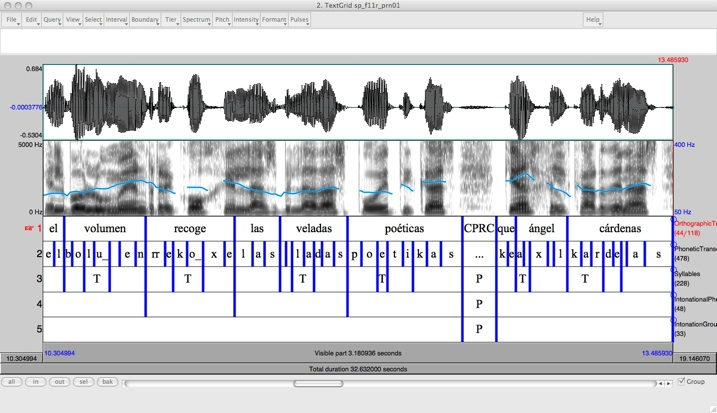
\includegraphics[width=\textwidth]{figures/GAR-img007.png}
\caption{Sample TextGrid containing the annotation of the Glissando corpus.}
\label{fig:gar:7}
\end{figure}

\section{Measurement and analysis}

The measurement and statistical analysis of the acoustic data from large corpora cannot be done manually either. Some current tools, such as Praat (for acoustic analysis) or R (for statistical processing), allow automation of these procedures by means of scripts. These tools allow the development of more complex tools for specific purposes, such as MelAn, which includes, in addition to the stylisation and annotation scripts, a set of Praat and R scripts for contour modelling (the extraction of intonation patterns from the input corpus, the calculation of their frequency, and the analysis of their relation to any higher level linguistic variable annotated in the corpus).

The modelling phase in MelAn allows the researcher to obtain two kinds of patterns: global, defined at Intonation Group (IG) level, which model the global evolution of P and V inflection points along the IG; and local, defined at Stress Group (SG) level, which represent the local shape of F0 patterns. \figref{fig:gar:8} illustrates this modelling scheme, with the P and V reference lines representing global patterns drawn on the F0 curve, and \figref{fig:gar:9} and \figref{fig:gar:10} present two examples of local final patterns and their corresponding inflection point labels.

  
\begin{figure}
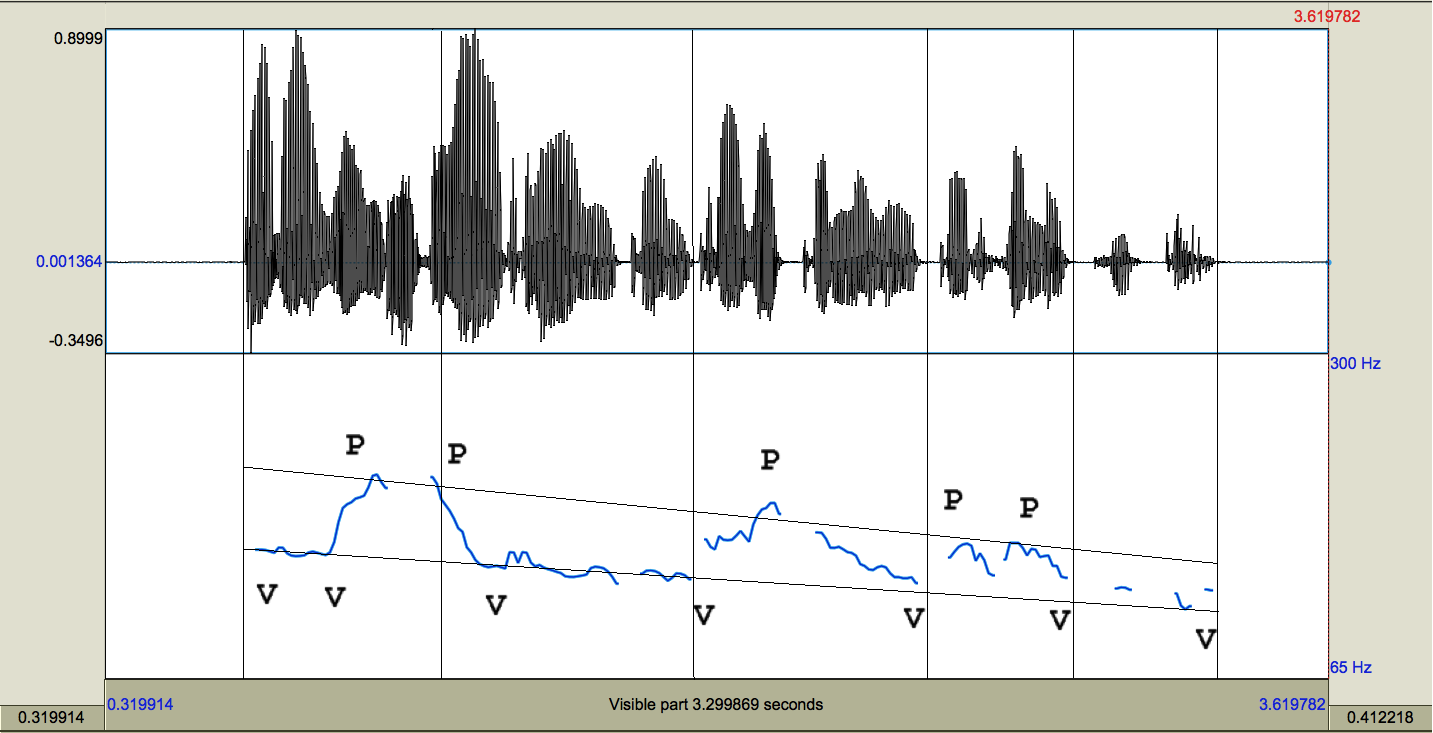
\includegraphics[width=\textwidth]{figures/GAR-img008.png}
\caption{Waveform and annotated F0 contour for the utterance ``Aragón se ha reencontrado como motor del equipo", uttered by a female speaker of Peninsular Spanish. Vertical lines indicate SG boundaries.}
\label{fig:gar:8}
\end{figure}

\begin{figure}
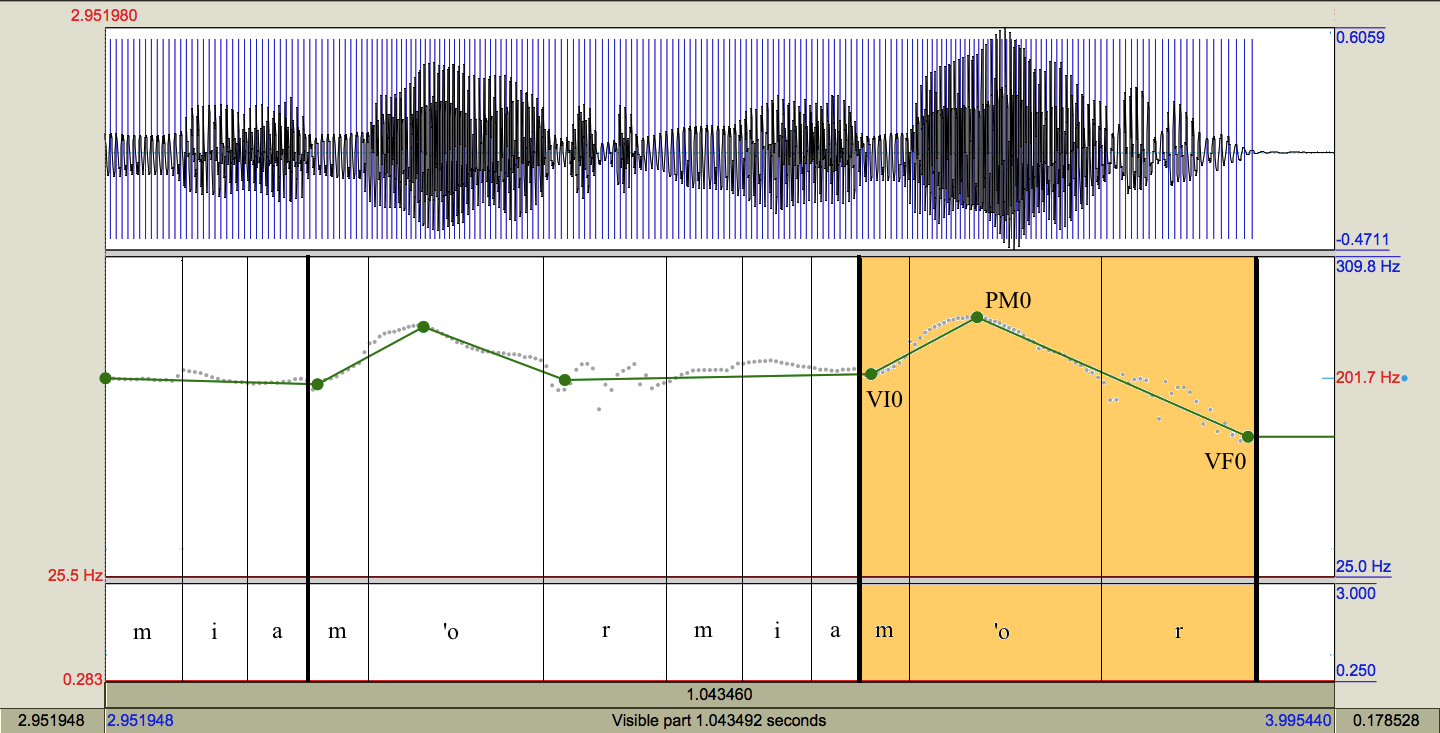
\includegraphics[width=\textwidth]{figures/GAR-img009.png}
\caption{Example of rise-fall pattern: VI0\_PM0\_VF0 \citep{Garrido2012enton}}
\label{fig:gar:9}
\end{figure}

\begin{figure}
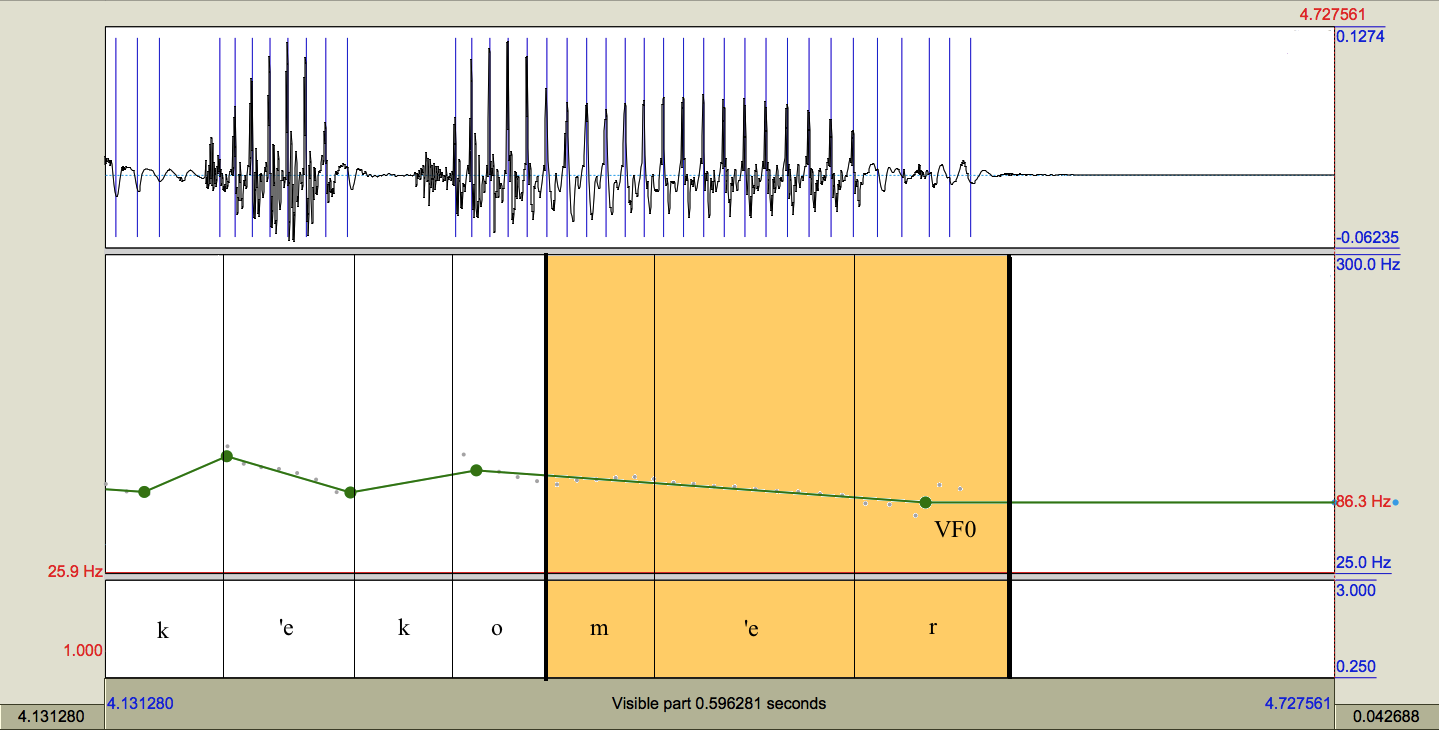
\includegraphics[width=\textwidth]{figures/GAR-img010.png}
\caption{Example of falling pattern: VF0 \citep{Garrido2012enton}}
\label{fig:gar:10}
\end{figure}

The output of this modelling procedure is twofold: first, a full inventory of local patterns in the input corpus for the different types of SG considered, with indication of their frequency in the analysed corpus (illustrated in \tabref{tab:gar:5}); and second, mean global patterns for the different considered IG types (\tabref{tab:gar:6}).

Local pattern labels presented in \tabref{tab:gar:5} are the result of concatenating the labels representing all the inflection points that make up the pattern. In addition, each inflection point label also includes two extra symbols to represent the position of the point with respect to the nucleus of its container syllable (``I'', for ``initial'', close to the beginning of the syllable nucleus; ``M'', for ``middle'', close to the centre of the nucleus; and ``F'', for ``final'', close to the end of the nucleus) and the syllable of the SG where the inflection point is located (``0'' if the syllable is the stressed one; ``1'' if the syllable is the one after the stressed one; and so on). For example, the label ``VI0\_PM0\_VF0'' used to describe the pattern illustrated in \figref{fig:gar:9}, indicates that this pattern is made up of three inflection points, all three located in the stressed syllable of the SG: the first one has V (``valley'') level, and is located close to the beginning of the syllabic nucleus; the second one has P (``peak'') level, and is close to the centre of the syllable nucleus; and finally, the third one also has V level, and is located in the vicinity of the end of the syllabic nucleus. In other terms, it is an example of a ``rise-fall'' F0 pattern.

\begin{table}
\begin{tabularx}{\textwidth}{Xrrrr}
\lsptoprule

Pattern & N of Syllables & Stressed Syllable & SG Position & N of Cases \\
\midrule
0 & 1 & 1 & INTERIOR & 382 \\
VI0\_PM0 & 1 & 1 & INTERIOR & 172 \\
PM0 & 1 & 1 & INTERIOR & 140 \\
PI0 & 1 & 1 & INTERIOR & 134 \\
VF0 & 1 & 1 & INTERIOR & 123 \\
0 & 2 & 1 & INTERIOR & 205 \\
PI0 & 2 & 1 & INTERIOR & 100 \\
PI1 & 2 & 1 & INTERIOR & 90 \\
VI0\_PM0 & 2 & 1 & INTERIOR & 82 \\
PM0 & 2 & 1 & INTERIOR & 69 \\
\lspbottomrule
\end{tabularx}
\caption{Simplified sample of an output file containing the list of extracted internal patterns obtained from the analysis of a part of the Glissando Catalan news subcorpus \citep{Garrido2013Glissando}. The ``INTERIOR'' label indicates that patterns appear in internal position within SG.}
\label{tab:gar:5}
\end{table}

\begin{samepage}

Global patterns presented in \tabref{tab:gar:6} represent the two mean reference lines calculated for each considered IG type (``INICIAL'', for initial IG within the sentence; ``FINAL'', for sentence final IG; ``INTERIOR'', for IG which are not initial nor final within the sentence; and ``INICIAL\_FINAL'', for IG which contain a whole sentence). Each reference line is defined by two values: the F0 value at the beginning of the reference line (which coincides with the beginning of the IG) and the mean slope of line. These lines can be calculated using Hertz or semitones as units and define the tonal range and register for each type of IG. This output can be used for different types of analyses, as illustrated by the studies described in the next sections.

\end{samepage}

\begin{sidewaystable}
\begin{tabularx}{\textwidth}{ll *{7}{S}}
\lsptoprule

Sentence Mood & IG Position & \pbox{1.3cm}{Number of Cases} & \pbox{1.3cm}{Mean Initial Value P} & \pbox{1.3cm}{Mean Final Value P} & \pbox{1.3cm}{Mean Slope P} & \pbox{1.3cm}{Mean Initial Value V} & \pbox{1.3cm}{Mean Final Value V} & \pbox{1.3cm}{Mean Slope V} \\
\midrule
ENUNCIATIVA & FINAL & 404 & 141.82 & 91.15 & -37.55 & 109.07 & 69.21 & -29.32\\
ENUNCIATIVA & INICIAL & 1946 & 149.52 & 109.80 & -22.92 & 112.97 & 85.06 & -12.05\\
ENUNCIATIVA & INICIAL\_FINAL & 363 & 158.91 & 90.57 & -45.30 & 120.27 & 69.18 & -33.74\\
ENUNCIATIVA & INTERIOR & 1823 & 137.50 & 106.15 & -18.17 & 108.13 & 80.72 & -14.78\\
EXCLAMATIVA & FINAL & 2 & 238.59 & 62.06 & -157.77 & 129.81 & 84.67 & -44.31\\
EXCLAMATIVA & INICIAL & 84 & 181.17 & 124.05 & -49.21 & 134.53 & 86.06 & -43.55\\
EXCLAMATIVA & INICIAL\_FINAL & 52 & 204.94 & 118.99 & -93.99 & 141.13 & 86.45 & -49.36\\
EXCLAMATIVA & INTERIOR & 5 & 186.84 & 99.35 & -81.39 & 139.53 & 80.26 & -55.74\\

\lspbottomrule
\end{tabularx}
\caption{Simplified sample of an output file containing the list of global F0 patterns obtained from the analysis of a part of the Glissando Catalan news subcorpus \citep{Garrido2013Glissando}. The ``INICIAL'', ``INTERIOR'', ``FINAL'' and ``INICIAL\_FINAL'' labels indicate the position of the IG within the sentence (initial, internal, final or initial and final at the same time, respectively).}
\label{tab:gar:6}
\end{sidewaystable}

\clearpage
\section{Using automatic techniques for the study of prosody: Some examples}

The next subsections present some examples of how this methodology has been applied to the study of prosody in different languages and conditions. All of these studies were carried out using the tools and methods described in the sections above.

\subsection{Analysis of pitch patterns in Spanish neutral speech}

The goal of the studies presented in \citep{Garrido2012enton,Garrido2012acent} was the description of the pitch patterns used in Spanish read neutral speech by different professional speakers, using a large corpus and a fully automatic procedure. The idea was to determine to what extent the use of automatic techniques could provide a reliable description of the intonation patterns which appear in a large corpus (actually, three different corpora of read speech collected for text-to-speech purposes, read by three different speakers, two women and a man, containing 33,730 internal and 11,460 final SG). The analysed material was automatically annotated using SegProso and MelAn, and a complete list of the patterns which appeared in non-final \citep{Garrido2012acent} and final \citep{Garrido2012enton} IG position was obtained. No manual revision of the resulting annotation was carried out.

Tables \ref{tab:gar:7}, \ref{tab:gar:8} and \ref{tab:gar:9}  present an excerpt of three of the obtained frequency lists, the ones corresponding to declarative, interrogative, and exclamative sentences, respectively.\largerpage

These lists were used to define a reduced set of the most frequent IG final intonation patterns, both at sentence-final and non-sentence-final position. Three main groups of patterns were defined: falling (\figref{fig:gar:11}), rising (\figref{fig:gar:12}), and rise-fall (\figref{fig:gar:13}). The most frequent patterns obtained are similar to the ones defined in previous studies using manual methodologies: in the case of falling patterns, for example, PI0\_VM0\_VF0 pattern (high F0 level at the beginning of the last stressed syllable of the intonation group, and F0 fall during the stressed syllable, which may finish at the end of the stressed syllable or in one of the post-stressed syllables, if there are any), the most frequent one in declarative sentences in the analysed corpus, is equivalent to the H+L* L\% tone in the ToBI framework, and VF0 (low F0 level along all the stressed syllable, and even beyond if there are post-stressed syllables), the second pattern in the frequency list for this sentence type, is equivalent to the L* L\% tone, reported to be one of the prototypical boundary tones for this sentence type in Spanish; for rising patterns, VI0\_PM0\_P+F0 pattern (low F0 level at the beginning of the final stressed syllable, followed by an F0 rise until the middle of the same syllable, to arrive at an even higher F0 level at the end of the stressed syllable), the most frequent one in interrogative sentences, would be equivalent to the L* HH\% boundary tone, considered prototypical of Spanish interrogative sentences (\citealt{EstebasVilaplanaPrieto.2008}). These patterns are also equivalent to the ones defined in Navarro’s classical study on Spanish intonation \citep{NavarroTomas.1944}.

\vfill
\begin{table}
% \fittable{
\begin{tabular}{lrrr}
\lsptoprule
Pattern & Number of Syllables SG & Sentence Mood & Number of Cases \\
\midrule
PI0\_VM0\_VF0 & 1 & AFIRM & 173 \\
VF0 & 1 & AFIRM & 171 \\
PI0\_VF0 & 1 & AFIRM & 130 \\
VI0\_PM0\_VF0 & 1 & AFIRM & 91 \\
VI0\_VF0 & 1 & AFIRM & 89 \\
PI0\_VI1\_VF1 & 2 & AFIRM & 198 \\
PI0\_VF0\_VF1 & 2 & AFIRM & 114 \\
VI1\_VF1 & 2 & AFIRM & 112 \\
PI0\_VI1\_VM1 & 2 & AFIRM & 80 \\
PI0\_VF0\_VM1 & 2 & AFIRM & 65 \\
PI0\_VI1\_VF2 & 3 & AFIRM & 13 \\
PI0\_VI1\_VM2 & 3 & AFIRM & 11 \\
PM0\_VI1\_VF2 & 3 & AFIRM & 9 \\
PI0\_VF0\_VM2 & 3 & AFIRM & 8 \\
PI0\_VF0\_VF2 & 3 & AFIRM & 7 \\
VI1\_VF2 & 3 & AFIRM & 7 \\
\lspbottomrule
\end{tabular}
% }
\caption{Most frequent sentence-final patterns in declarative sentences \citep{Garrido2012enton}}
\label{tab:gar:7}
\end{table}
\vfill

\begin{table}
% \fittable{
\begin{tabular}{lrrr}
\lsptoprule
Pattern & Number of Syllables SG & Sentence Mood & Number of Cases \\
\midrule
VI0\_PM0\_P+F0 & 1 & INT & 29 \\
VI0\_PF0 & 1 & INT & 19 \\
VM0\_PF0 & 1 & INT & 17 \\
PI0\_VF0 & 1 & INT & 16 \\
VI0\_PM0\_VF0 & 1 & INT & 16 \\
VI1\_PF1 & 2 & INT & 23 \\
VI1\_PM1 & 2 & INT & 21 \\
VI1\_PM1\_P+F1 & 2 & INT & 17 \\
VI1\_PM1\_PF1 & 2 & INT & 15 \\
PI0\_VI1\_VF1 & 2 & INT & 11 \\
VI0\_VI1\_PM1\_P+F1 & 2 & INT & 11 \\
VM1\_PM2 & 3 & INT & 2 \\
\lspbottomrule
\end{tabular}
% }

\caption{Most frequent sentence-final patterns in interrogative sentences \citep{Garrido2012enton}}
\label{tab:gar:8}
\end{table}

\begin{table}
\fittable{
\begin{tabular}{lrrr}
\lsptoprule
Pattern & Number of Syllables SG & Sentence Mood & Number of Cases \\
\midrule
VI0\_VF0 & 1 & ADM & 11 \\
VI0\_PM0\_VF0 & 1 & ADM & 9 \\
0 & 1 & ADM & 8 \\
PI0\_VF0 & 1 & ADM & 6 \\
PI0\_VM0\_VF0 & 1 & ADM & 6 \\
VI0\_VM1 & 2 & ADM & 4 \\
PI0\_VI1\_VF1 & 2 & ADM & 3 \\
PI0\_VI1\_VM1 & 2 & ADM & 3 \\
PM0\_VM1 & 2 & ADM & 3 \\
PM0\_VM1\_VF1 & 2 & ADM & 3 \\
VI0\_PM0\_PI1\_VM1 & 2 & ADM & 3 \\
VI0\_PM0\_PI1\_VM1\_VF1 & 2 & ADM & 3 \\
VI1\_VM1 & 2 & ADM & 3 \\
VM0\_VF1 & 2 & ADM & 3 \\
\lspbottomrule
\end{tabular}
}
\caption{Most frequent sentence-final patterns in exclamative sentences \citep{Garrido2012enton}}
\label{tab:gar:9}
\end{table}

  
%%please move the includegraphics inside the {figure} environment
%%\includegraphics[width=\textwidth]{GAR-img25.png}
 

\begin{figure}
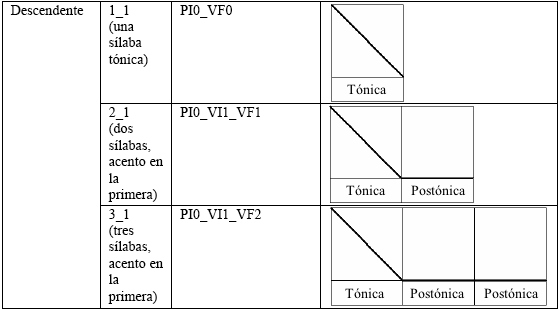
\includegraphics[width=.8\textwidth]{figures/GAR-img011-1.png}
\caption{MelAn labels and schematic representation of the most frequent sentence-final falling (``descendente'') patterns \citep{Garrido2012enton}.}
\label{fig:gar:11}
\end{figure}

  
%%please move the includegraphics inside the {figure} environment
%%\includegraphics[width=\textwidth]{GAR-img26.png}
 

\begin{figure}
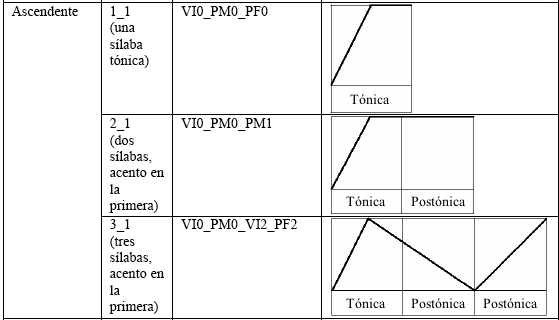
\includegraphics[width=.8\textwidth]{figures/GAR-img012-1.png}
\caption{MelAn labels and schematic representation of the most frequent sentence-final rising (``ascendente'') patterns \citep{Garrido2012enton}.}
\label{fig:gar:12}
\end{figure}\clearpage

  
%%please move the includegraphics inside the {figure} environment
%%\includegraphics[width=\textwidth]{GAR-img27.png}
   
%%please move the includegraphics inside the {figure} environment
%%\includegraphics[width=\textwidth]{GAR-img28.png}
 

\begin{figure}
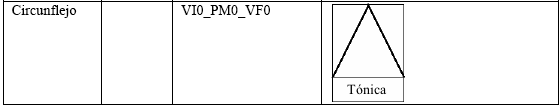
\includegraphics[width=.8\textwidth]{figures/GAR-img013-1.png}   
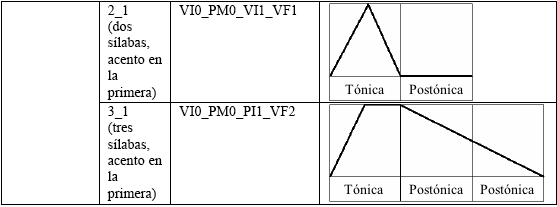
\includegraphics[width=.8\textwidth]{figures/GAR-img014-2.png}
\caption{MelAn labels and schematic representation of the most frequent sentence-final rise-fall (``circunflejo'') patterns \citep{Garrido2012enton}.}
\label{fig:gar:13}
\end{figure}

The results show that the employed methodology was useful to obtain reliable results in intonation analysis from large collection of data. In addition, MelAn labels allow for the description of intonation patterns in more detail than other annotation conventions, as they provide information about the number of inflection points in the pattern, its relative height (peak or valley), and its location within SG. This level of detail enables the researcher to distinguish, for example, between the VI0\_PM0\_P+F0 pattern, which is the prototypical final pattern for interrogative sentences, as stated before, and VI0\_PM0\_PF0 (``continuation rise'' pattern), in which the final F0 reaches a lower F0 height than in the previous one (P instead of P+), and which is the rising pattern that is typical of non-final intonation groups. Both patterns are labelled in the ToBI framework with the same L* HH\% label. Finally, the lists of patterns obtained with MelAn provide much more information about the variety of intonation patterns used in a large corpus, something very difficult to achieve when analyzing small corpora by manual means.

The results presented in \tabref{tab:gar:9} also illustrate one of this methodology’s drawbacks: when the analyzed data is scarce, as in this case with the number of exclamative sentences in the corpus, the distribution of the observed patterns shows some dispersion and no clear tendencies are observed in their frequency of use.

\subsection{Analysis of pitch patterns in Mandarin Chinese}\largerpage[2.5]

The study described in \citet{Yao2015} is an example of the application of this methodology to a language different from Spanish, and to a prosodic phenomenon different from intonation. The goal of this work was the description of the phonetic realisation of tones in Mandarin Chinese, using a corpus of isolated utterances and paragraphs, recorded by nine different native speakers of Mandarin Chinese, three men and six women (651 sentences, 15,873 syllables in total). Adapted versions of SegProso and MelAn were used to annotate all syllables in the corpus (the natural domain for tones), and to obtain a list of the most frequent pitch patterns associated to the tones defined in classical studies of Mandarin Chinese. In this case, as no automatic phonetic aligner for Mandarin Chinese was available, phonetic transcription in Praat was done manually.

\tabref{tab:gar:10} summarizes the results of the analysis of these lists, showing which of the five F0 patterns were most frequently observed for tones 1, 2, 3 and 4, the number of times that they appeared in the corpus, and their relative frequency within the total number of analysed syllables showing that tone. In this case, as the patterns cover one single syllable, the pattern labels are made up only by the concatenation of the labels of each detected inflection point, with no label to indicate the syllable number. The ``0'' label indicates that no inflection point was detected within the syllable. The results seem to indicate that canonical pitch shapes of Chinese tones may present some ``alotonic'' variants, with different possible shapes for each theoretical realisation. So, for example, tone 1, which is described in classical studies of Mandarin Chinese as a ``high'' tone \citep{Chao1922} presents most frequently in patterns containing one or two ``P'' inflection points, but also as a variant with an initial low inflection point, followed by a high inflection point in the middle of the syllabic nucleus (VI\_PM). 

\begin{table}
\footnotesize
\begin{tabularx}{\textwidth}{X lrr lr}
\lsptoprule
Tone & Pattern & Frequency & Tone & Pattern & Frequency\\
\midrule 
1 (2799) & PI & 28,76 (805) & 3 (2602) & VM & 15,37 (400) \\
& 0 & 24,90 (697) &  & 0 & 12,07 (314) \\
& VI\_PM & 8,75 (245) &  & PI\_VM & 11,80 (307) \\
& PF & 7,15 (200) &  & VI & 10,11 (263) \\
& PI\_PF & 6,07 (170) &  & VF & 5,38 (140) \\
\tablevspace
2 (3347) & VM & 21,84 (731) & 4 (5805) & PI & 27,46 (1594) \\
& 0 & 18,29 (612) &  & 0 & 12,16 (706) \\
& VI & 11,41 (382) &  & PI\_VF & 10,30 (598) \\
& VF & 6,66 (223) &  & PM & 7,44 (432) \\
& PI\_VM & 6,54 (219) &  & PI\_VM & 6,74 (391) \\ 
\lspbottomrule
\end{tabularx}
\caption{Most frequent pitch patterns in the four analysed tones \citep{Yao2015}}
\label{tab:gar:10}
\end{table}

\largerpage[2.5]The use of MelAn to process this large sample of acoustic data (thousands of syllables for each analysed tone) allowed for the description of the phonetic variation of the linguistic speech patterns, a fact which is much more difficult to detect and describe using manual methodologies.\largerpage

\subsection{Analysis of pitch patterns in Spanish emotional speech} 

MelAn and SegProso tools were used in \citet{Garrido2011} to automatically annotate the INTERFACE corpus \citep{Hozjan2002}, a corpus of Spanish emotional speech read by two professional actors, a woman and a man, imitating different emotional states (joy, disgust, anger, fear, surprise, sadness, and neutral). The corpus was not fully analysed for this study, only a subset of 5,859 utterances, representing the six considered emotions (4,201) and the neutral state (1,658).  The inventory of pitch patterns provided by MelAn allowed for the analysis of the most frequent patterns associated to each emotion (\tabref{tab:gar:11} and \tabref{tab:gar:12}). As illustrated in these tables, the number of items for the most frequent patterns is rather small, and some variation is observed in the data. 



\begin{table}[p]

\begin{tabular}{llrlr}
\lsptoprule

Emotion  & Male Speaker  & \pbox{1cm}{N} & Female Speaker & \pbox{1cm}{N} \\
\midrule
Joy      & VI0\_PM0\_VF0 (C) & 11              & VF0 (D)                & 7               \\
         & 0                 & 5               & VI0\_PM0\_VF0 (C)      & 5               \\
         & VF0 (D)           & 5               & 0                      & 4               \\
         &                   &                 & VI0\_PM0\_PF0 (A)      & 4               \\
         &                   &                 & VI0\_V-M0 (D)          & 4               \\
\midrule
Disgust  & 0                 & 7               & VF0 (D)                & 9               \\
         & VI0\_PM0\_VF0 (C) & 5               & VI0\_PM0\_VF0 (C)      & 5               \\
         & VM0 (D)           & 5               & PI0\_VM0\_PF0 (A)      & 4               \\
         &                   &                 & PI0\_VM0\_VF0 (D)      & 4               \\
         &                   &                 & VI0\_PI0\_VM0\_PF0 (A) & 4               \\
\midrule
Anger    & 0                 & 5               & VF0 (D)                & 11              \\
         & VM0 (D)           & 4               & 0                      & 7               \\
         & VF0 (D)           & 3               & PI0\_VM0\_VF0 (D)      & 5               \\
         &                   &                 & VI0\_V-F0 (D)          & 5               \\
\midrule
Fear     & VI0\_PM0\_VF0 (C) & 18              & VF0 (D)                & 14              \\
         & PM0\_VF0 (D)      & 8               & VI0\_PM0\_VF0 (C)      & 9               \\
         & 0                 & 5               & 0                      & 8               \\
\midrule
Surprise & VI0\_PM0\_VF0 (C) & 19              & VI0\_PM0\_VF0 (C)      & 27              \\
         & VI0\_PM0\_PF0 (A) & 6               & VI0\_PF0 (A)           & 5               \\
         & PM0\_VF0 (D)      & 5               & VI0\_PM0\_PF0 (A)      & 4               \\
\midrule
Sadness  & 0                 & 9               & 0                      & 6               \\
         & PI0\_VM0\_PF0 (A) & 5               & PF0 (A)                & 6               \\
         & VM0 (D)           & 5               & PI0\_VM0\_VF0 (D)      & 6               \\
         &                   &                 & VI0\_PM0\_PF0 (A)      & 6               \\
\midrule
Neutral  & VM0 (D)           & 17              & VF0 (D)                & 44              \\
         & VI0\_VM0 (D)      & 13              & VI0\_VF0 (D)           & 15              \\
         & VF0 (D)           & 12              & VM0 (D)                & 13             \\
         \lspbottomrule
\end{tabular}
\caption{Most frequent pitch patterns in the 1-syllable final (sentence final) SG, both for neutral and emotional speech \citep{Garrido2011}.}
\label{tab:gar:11}
\end{table}



\begin{table}[p]
\begin{tabular}{llrlr}
\lsptoprule
Emotion  & Male Speaker           & N & Female Speaker          & N \\
\midrule
Joy      & 0                      & 8               & VI0\_VM1 (D)            & 8               \\
         & VI0\_PF0\_PI1\_VM1 (C) & 7               & VM1 (D)                 & 7               \\
         & VI0\_PM0\_PI1\_VM1 (C) & 6               & VI0\_PM0\_VM1 (C)       & 6               \\
         &                        &                 & VI0\_VF1 (D)            & 6               \\
\midrule
Disgust  & 0                      & 12              & VI0\_VM1 (D)            & 9               \\
         & VI0\_PM0\_VF0 (C)      & 9               & 0                       & 8               \\
         & VI1 (D)                & 9               & VM1 (D)                 & 7               \\
\midrule
Anger    & VF0 (D)                & 5               & VM1 (D)                 & 16              \\
         & VI0\_PM0\_VM1 (C)      & 4               & VF1 (D)                 & 11              \\
         & VI0\_PM0\_VI1 (C)      & 3               & VI0\_VM1 (D)            & 9               \\
         & VI0\_VF0 (D)           & 3               &                         &                 \\
         & VI1 (D)                & 3               &                         &                 \\
\midrule
Fear     & VI0\_PM0\_PI1\_VF1 (C) & 11              & 0                       & 13              \\
         & VI0\_PM0\_VI1\_VF1 (C) & 9               & VI0\_PM0\_VM1 (C)       & 11              \\
         & 0                      & 7               & VM1 (D)                 & 11              \\
         & VI0\_PM0\_PI1\_VM1 (C) & 7               &                         &                 \\
\midrule
Surprise & VI0\_PM0\_PI1\_VM1 (C) & 7               & VI0\_PM0\_PI1\_VM1 (C)  & 13              \\
         & VI0\_PM0\_PI1 (A)      & 6               & VI0\_PF0\_PI1\_VM1 (C)  & 10              \\
         & VI0\_PM0\_PI1\_P+M1    & 5               & VI0\_PF0\_VM1 (C)       & 7               \\
         & (A)                    &                 & VI0\_PM0\_VM1\_VF1 (C)  & 7               \\
\midrule
Sadness  & PI0\_VM0\_PI1 (A)      & 9               & PI0\_VM0\_VI1\_PM1\_PF1 & 6               \\
         & 0                      & 8               & (A)                     & 6               \\
         & PF0 (A)                & 6               & PI1\_VM1 (D)            & 6               \\
         & PM0\_VF0 (D)           & 6               & PM1 (A)                 &                 \\
\midrule
Neutral  & PI0\_VI1\_VM1 (D)      & 32              & VM1 (D)                 & 30              \\
         & VI1 (D)                & 24              & VF1 (D)                 & 25              \\
         & 0                      & 15              & VI0\_VM1 (D)            & 25  \\
\lspbottomrule         
\end{tabular}
\caption{Most frequent pitch patterns in the 2-syllable final (sentence final) SG, both for neutral and emotional speech \citep{Garrido2011}.}
\label{tab:gar:12}
\end{table}


A similar study, also aimed at describing the pitch patterns associated with the expression of emotions in Spanish, is described in \citet{Laplaza2014}, but in this case, the corpus was much smaller (only 525 utterances, read by a professional actor imitating the different intended emotions, 21 in this case, so there were only 25 utterances representing each emotion). The results, if analysed separately by emotion, showed a large dispersion of the patterns, which was interpreted as an indication that much larger corpora were needed to obtain significant data about most patterns when using this methodology. For this reason, pitch patterns were not described separately for each emotion, but only for comparing emotional and non-emotional utterances (\tabref{tab:gar:13}).



These two studies illustrate once more that the results may show some dispersion when the size of the corpus is not large enough. This was even clearer in the case of the second corpus, with only 25 utterances for each of the 21 analysed emotions, so the obtained patterns had to be reanalysed not considering emotion as a discriminating variable to get more significant results.

Despite this fact, the patterns observed in both studies were consistent with previous descriptions of Spanish emotional speech, such as the one by \citet{NavarroTomas.1944}, in which the use of a ``rise-fall'' final pattern was considered to be a typical mark of emotional speech, but coexisting with other falling and rising patterns. This ``rise-fall'' pattern described by Navarro coincides with the VI0\_PM0\_VF0 pattern (low F0 level at the beginning of the stressed syllable, F0 peak in the middle of the same syllable, and low F0 level again at the end of the same syllable) observed among the most frequent patterns in both studies, but coexisting with other falling (VF0) and rising patterns (VI0\_PM0\_PF0). The results presented in \tabref{tab:gar:11} show also that this ``rise-fall'' pattern is used to express only some emotions, such as joy, disgust, surprise, or fear. Anger and sadness did not illustrate this pattern.
\begin{table}[p]
\footnotesize
\begin{tabularx}{\textwidth}{lXXXX} 
\lsptoprule
& \multicolumn{2}{c}{Non-sentence final} &  \multicolumn{2}{c}{Sentence final} \\\cmidrule(lr){2-3} \cmidrule(lr){4-5}
{Condition} & {1 syllable} & {2 syllable} & {1 syllable} & {2 syllable} \\\midrule
{Neutral} & {VI0\_PM0\_PF0} 

{VI0\_PM0\_VF0} 

{VI0\_PF0} 

{PI0\_VF0} 

PF0 & {PI0\_VI1\_VM1} 

{0} 

{PM0\_VI1\_VM1} 

{PI0\_VI1\_VF1} 

VI1\_PM1 & {VF0} 

{VI0\_VF0} 

{PI0\_VM0} 

{VM0} 

VI0\_VM0 & {PI0\_VI1\_VM1} 

{VM1} 

{VI1\_VM1} 

{PI0\_VF0\_VM1} 

PI0\_VM1 \\
{Emotional} & {0} 

{VF0} 

{VI0\_PM0\_VF0} 

{PF0} 

PI0\_VF0 & {PI0\_VM1} 

{VI0\_PI1\_VF1} 

{PM0\_VM1\_PF1} 

{PM1\_VF1} 

\mbox{VI0\_PF0\_VM1\_VF1} & {VF0} 

{VI0\_PF0} 

{VI0\_PM0\_VF0} 

{VI0\_VF0} 

VI0\_PM0\_PF0 & {VM1} 

{VI0\_VM1} 

{PI0\_VM1} 

{VF1} 

PI1\_VM1 \\
\lspbottomrule
\end{tabularx}


\caption{Most frequent pitch patterns in the 1-syllable and 2-syllable final (non-sentence final and sentence final) SG, both for neutral and emotional speech (\citealt{Laplaza2014}).}
\label{tab:gar:13}
\end{table}

\begin{table}[p]
\fittable{
\begin{tabular}{lrrrr}
\lsptoprule
Pattern & Number of Syllables SG & Stressed Syllable & Speech mood & Number of cases\\
\midrule 
PF0 & 1 & 1 & ENUNCIATIVA & 6\\
VI0\_PF0 & 1 & 1 & ENUNCIATIVA & 6\\
PI0 & 1 & 1 & ENUNCIATIVA & 3\\
VF0 & 1 & 1 & ENUNCIATIVA & 3\\
VI1 & 2 & 1 & ENUNCIATIVA & 5\\
VI0\_PM0\_PM1 & 2 & 1 & ENUNCIATIVA & 4\\
PI0\_VF1 & 2 & 1 & ENUNCIATIVA & 3\\
PI0\_VI1\_PM1 & 2 & 1 & ENUNCIATIVA & 3\\
\lspbottomrule
\end{tabular}
}

\caption{Most frequent patterns appearing in sentence-final position (\citealt{GarridoRustullet2011}). The ``ENUNCIATIVA'' label indicates that patterns appear in declarative sentences.}
\label{tab:gar:14}
\end{table}\clearpage

\subsection{Analysis of pitch patterns in Spanish dialogues}

Finally, the analysis described in \citet{GarridoRustullet2011} provides an example of the application of this methodology to the analysis of pitch patterns in Spanish dialogue speech. The analysed material consisted of four dialogues between two radio professional speakers and extracted from the Glissando corpus: three task oriented dialogues (one about travel information, one about university information, and the last about tourist information), and one informal dialogue, with a total duration of 22 minutes and 53 seconds (2,964 analysed SG). 


In this case as well, the analysed material was not very large, and again, the dispersion of the data was noticeable, as shown in \tabref{tab:gar:14}, which presents the observed sentence-final pitch patterns for declarative sentences: although some patterns appeared more frequently than others, the number of items for each detected pattern was quite small, and the differences were not clear enough to extract general conclusions.

\section{Conclusions}

The experiments outlined in the previous sections seem to indicate that the use of fully automatic tools (such as MelAn) to process intonation can provide results that are comparable with the ones obtained by manual techniques, and offer new possibilities for the study of prosodic variation, as they enable researchers to obtain the full inventory of intonation patterns present in a corpus with detailed information about the frequency of each one.

However, input data has to be large enough to obtain a significant number of examples of each observed pattern and to get reliable results about the relative frequency of each pattern. The challenge, then, is to collect the necessary amount of speech to obtain reliable results, something that is difficult to do with classical corpus recording approaches, as was the case with the analyses of emotional speech, in which the number of utterances which represented each emotion was rather small.

At any rate, corpus-based techniques are a clear challenge for prosody research in the future, and even now, they can be used to carry out relevant research if a significant amount of speech material is available for analysis. There is a large number of automatic tools to complete the different tasks associated to the experimental analysis of prosody (corpus collection, corpus annotation, measurement and analysis), although in some specific steps, such as orthographic transcription, manual work seems still unavoidable. The accuracy of these tools, although it is not perfect, seems to be high enough to consider their use even without manual post-processing of the data, if the amount of speech data available for analysis is sufficient, and the noise introduced by the automatic tools can be balanced with the quantity of processed data. Or at least, these tools can drastically reduce the time devoted to manual annotation.

Such a corpus-based, ``big data'' approach to the analysis of prosody offers new methodological ways, as already mentioned, for the study of prosodic invariance, a classical problem in phonetic and phonological description of prosody: prosodic invariance can be established by analysing the speech of many different speakers, not only two or three, offering a much higher description power. But it is also a challenge for the study of prosodic variation at all levels (geographical, situational, intra, and interspeaker).

It is evident, however, that this approach presents still some important problems: for example, in many cases it is still difficult to obtain such a large amount of speech for analysis, especially in the case of endangered or minority languages, and with an acoustic quality that makes it suitable for automatic processing; and more complex and accurate tools are necessary, in order to improve the reliability of the annotated data used for analysis. But it seems clear that current research on speech technology and phonetics will provide such tools in the near future, and these corpus-based methodologies will become the norm in prosody analysis, as well as in other disciplines dealing with speech processing.

\section*{Acknowledgements}

I would like to show my gratitude to Kimber Fodge for her help with the review of this chapter.

\sloppy
\printbibliography[heading=subbibliography,notkeyword=this]

\end{document}
